\section{Learning}
\label{sec:learning}
As mentioned earlier, the branching factor of O-MCTS increases when the number
of options increases. When many options are defined, exploring all the options
when an option has finished becomes infeasible. By estimating
\emph{option values}, the mean and variance of the expected return of an option,
we can detect which options should be explored.

The return $R_o$ for using option $o$ from timestep $t$ to $t+n$ is calculated
by adding the discounted rewards $r_t$ for all of the states visited by that
option.  $$R_o = r_{t} + \gamma r_{t+1} + \gamma^2 r_{t+2} + \cdots + \gamma^n
r_{t+n},$$ where $\gamma \in [0, 1]$ is the discount rate parameter, which
influences the importance of rewards that lay further in the future: an option
with reward 1 at timestep $t$ will get a greater return than an option with the
same reward at timestep $t+1$.  

The set of options consists of different options of the same \emph{type}. For example,
there is an option for going to a movable sprite, which has type
\texttt{GoToMovableOption}. An instance of this option exists for each movable
sprite in the game. \emph{Subtypes} are defined as well. In this case, each
unique game sprite has its own subtype. The mean and variance of the options'
discounted rewards are kept per subtype. Each time an option is finished, its
subtype's values $\mu_o$ and $\sigma_o$ are updated by respectively taking the
mean and variance of all the returns of this subtype. By saving values per
subtype the algorithm can regularize over unique sprites.

\begin{algorithm}
	\caption{$\mathsf{OL-MCTS}(O, r, t, d, v, \mu, \sigma)$}
	\label{alg:olmcts}
	\begin{algorithmic}[1]
		\State $C_{s \in S} \gets \emptyset$
		\State $\mathbf{o} \gets \emptyset$
		\While {$time\_taken < t$} \label{alg:olmcts:mainloop}
			\State $s \gets r$
			\While {$\neg \mathsf{stop}(s, d)$} \label{alg:olmcts:innerloop}
				\If{$s \in \beta(o_s)$} \label{alg:olmcts:sp}
					\State $\mathsf{update\_values}(s, o_s, \mu, \sigma)$ \Comment{Update $\mu$ and $\sigma$}
					\State $\mathbf{p}_s \gets \cup_o (s \in I_{o \in O})$
				\Else
					\State $\mathbf{p}_s \gets \{o_s\}$
				\EndIf \label{alg:olmcts:scs}
				\State $\mathbf{m} \gets \cup_o (o_{s \in \mathbf{c}_s})$
				\If{$n_s < v$} \Comment{Apply \textsf{crazy\_stone}}
					\State $\mathbf{u}_s \gets \mathsf{crazy\_stone}(\mu, \sigma, \mathbf{p}_s)$
					\State $\omega \gets \mathsf{weighted\_random}(\mathbf{u}_s, \mathbf{p}_s)$
					\If{$\omega \not\in \mathbf{m}$} \Comment{option $\omega$ not expanded}
						\State $a \gets \mathsf{get\_action}(\omega, s)$ 
						\State $s' \gets \mathsf{expand}(s, a)$ 
						\State $\mathbf{c}_s \gets \mathbf{c}_s \cup \{s'\}$
						\State $o_{s'} \gets \omega$
						\State \textbf{break}
					\Else
						\State $s' \gets s \in \mathbf{c}_s : o_s = \omega$
					\EndIf

				\Else \Comment{Apply \textsf{uct}}
					\State $s' \gets \mathsf{uct}(s)$ \label{alg:olmcts:uct}
				\EndIf \label{alg:olmcts:ecs}
				\State $s \gets s'$ \label{alg:olmcts:ss}
			\EndWhile
			\State $\delta \gets \mathsf{rollout}(s')$ \label{alg:olmcts:rollout}
			\State $\mathsf{back\_up}(s', \delta)$ \label{alg:olmcts:backup}
		\EndWhile
	\end{algorithmic}
\end{algorithm}
\begin{figure}
	\centering
	%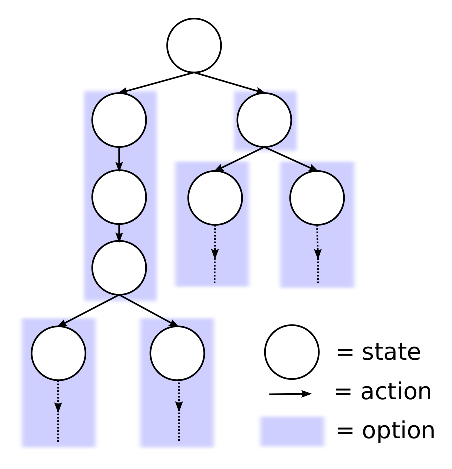
\epsfig{file=includes/omcts.eps, width=.5\columnwidth}
	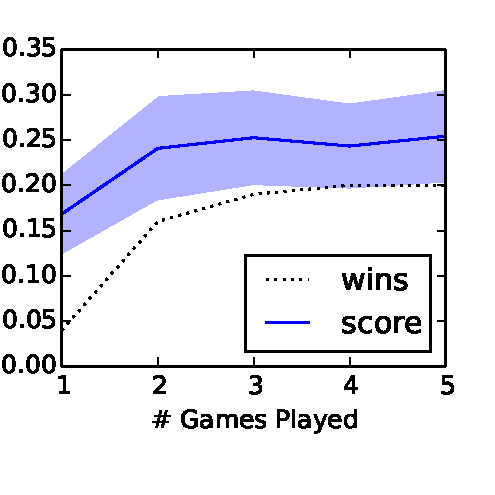
\includegraphics[width=\columnwidth]{includes/learning}
	\caption{Shows average improvement of the OL-MCTS on game x when playing 5
		games in a row for 20 times}
	\label{fig:learning-results}
\end{figure}

Now we have an option value and variance we can use the crazy stone algorithm
to reduce calculation time by shifting the focus of the exploration to promising
options. This means that not all children of a node will be expanded, but only
the ones selected by crazy stone. The algorithm then changes to algorithm
\ref{alg:olmcts}. Most of it is the same, with the exception that crazy stone
selects what node to expand in the first $v$ node visits. Because crazy stone
can select the same option several times, this prevents the algorithm from
expanding all the children, which saves time. 

Crazy stone uses the mean return $R_o$ of each option as its estimated value
$\mu$ for selecting which option to select or expand. After a predefined number
of visits $v$ to a node, the selection strategy $\mathsf{uct}$ is followed to
tweak the option selection.



The information learned in a game can be transferred if the game is played
again by supplying OL-MCTS with the $\mu$ and $\sigma$ of the previous game. We
will refer to this as \emph{Option Tranfer Learning MCTS (OTL-MCTS)}.
